\documentclass[a4paper,10pt]{article}
\usepackage[utf8x]{inputenc}


%preamble
\usepackage{amsmath}
\usepackage{amssymb}
\usepackage{amsthm}
\usepackage{mathtools}
% \usepackage{lineno,hyperref}
 \usepackage{fullpage}
\usepackage{slashed}	%feynman slashed symbols
\usepackage{verbatim}
\usepackage{graphicx}
\usepackage{bm}
\usepackage{subfigure}
\usepackage{relsize}	%scalable math
\usepackage{threeparttable}
\usepackage{array}
\usepackage{color}
\usepackage{hhline}
\usepackage{multirow}
% \usepackage{fancyhdr}

%

% \pagestyle{fancy}
%\headheight 0in
%\headset 0.25in

%  \rhead{}
%\rfoot{Right botton}
%\lfoot{Left bottom}
% \cfoot{\thepage}

\setlength{\topmargin}{0in}
\setlength{\headheight}{0in}
\setlength{\headsep}{25pt}
\setlength{\voffset}{-0.25in}
\parskip 5.0pt	  % sets spacing between paragraphs
\parindent 10pt	  % sets leading space for paragraphs

%%---------------------------------------
%% commands from HamiltonianofLightConeQCD.tex
\newcommand{\comments}[1] {}
\newcommand{\dd} {\mathrm{d}} %% derivative in integral measure
\newcommand{\half}[1][1] {\mathsmaller{\frac{#1}{2}}}
\newcommand{\tr} {\textbf{Tr}}
\newcommand{\imag} {\text{i}} %unite of imaginary number
\newcommand{\bra}[1] {\left< #1 |\right.}
\newcommand{\ket}[1] {\left.| #1 \right> }
\newcommand{\abs}[1] {{\left| #1 \right|}}

\def\dbar{{\mathchar'26\mkern-12mu \mathrm{d}^2}}

% make roman numerals
\makeatletter
\newcommand{\rmnum}[1]{\romannumeral #1}
\newcommand{\Rmnum}[1]{\expandafter\@slowromancap\romannumeral #1@}
\makeatother
\date{}

%opening
\title{Talmi-Moshinsky Transformation for 2D Harmonic Oscillator Functions}
\author{Yang Li \\
\textit{Department of Physics and Astronomy, Iowa State University, Ames IA 50011} \\
\texttt{leeyoung@iastate.edu} \\
(Dated: \today)
}

\begin{document}

 \maketitle

\paragraph{The Harmonic Oscillator Functions} The harmonic oscillator (HO) functions are the eigenstate wave function of the 
Hamiltonian 
\begin{equation}
  H = \frac{1}{2m}\bm p^2 + \frac{1}{2} m\omega^2 \bm r^2,
\end{equation}
where $\bm r$ and $\bm p$ are the coordinate and momentum operator, respectively, $[r_i, p_j] = i\delta_{ij}$. It is convenient
to introduce a new parameter $b = \sqrt{m\omega}$ (here we take $\hbar = c =1$), called the basis energy scale. $\ell = b^{-1}$ 
is called the natural length of the HO functions.

In the momentum representation, the eigenstate wavefunctions read, 
\begin{equation}\label{eq2}
 \psi^m_{n}(\bm p) \equiv b^{-1} \sqrt{\frac{4\pi n!}{(n+|m|)!}} \rho^{|m|} e^{-\frac{1}{2}\rho^2} L_n^{|m|}(\rho^2) e^{im\theta},
\end{equation}
where $\rho = |\bm p|/b$, $\theta = \arg \bm p$, $L_n^\alpha(x)$ are the generalized Laguerre polynomials.
%
\begin{figure}
 \centering 
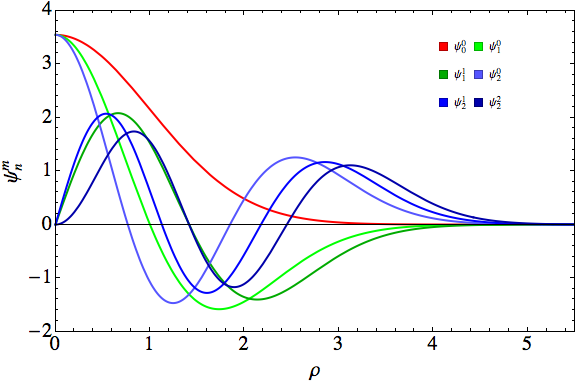
\includegraphics[width=.5\textwidth]{HOF}
\caption{The first few HO functions ($\theta = 0$)}
\end{figure}
%
This definition of the HO functions satisfies the orthonormality relations: 
\begin{align}\label{orthonormality}
 \int \frac{\mathrm{d}^2\bm p}{(2\pi)^2} {\psi_n^m}^*(\bm p)\psi_{n'}^{m'}(\bm p) &= \delta_{nn'}\delta_{mm'}, \\
 \sum_{n=0}^{+\infty} \sum_{m=-n}^n \psi_n^m(\bm p) \psi_n^m(\bm p') &= (2\pi)^2\delta^{(2)}(\bm p-\bm p').
\end{align}

\paragraph{The Jacobi Variables}
Consider a two-body system. Let $\bm p_1$, $\bm p_2$ be the momentum of the two particles respectively, and 
$m_1$ and $m_2$ be the mass of the two particles respectively. 
The total momentum $\bm P = \bm p_1 + \bm p_2$. The relative momentum is $\bm p = \frac{m_2}{m_1+m_2}\bm p_1 - \frac{m_1}{m_1+m_2}\bm p_2$.
The total mass $M = m_1+m_2$. The reduced mass $m = \frac{m_1m_2}{m_1+m_2}$. Similarly, the center-of-mass coordinate 
is $\bm R = \frac{m_1}{m_1+m_2}\bm r_1 + \frac{m_2}{m_1+m_2}\bm r_2$. The relative coordinate is $\bm r = \bm r_1-\bm r_2$.
It is easy to see $[R_i, P_j] = i\delta_{ij}$ and $[r_i, p_j] = i\delta_{ij}$, $[R_i, p_j]=[r_i,P_j]=0$, i.e. $\bm R$ is conjugate to $\bm P$ and 
$\bm r$ to $\bm p$. The procedure can be generalized to the $n$-body system. The resulted coordinates and momenta are called the Jacobi 
variables.

The generating Hamiltonian of the two particle system 
\begin{equation}
   H = \frac{1}{2m_1}\bm p^2_1 + \frac{1}{2} m_1\omega^2 \bm r^2_1 + \frac{1}{2m_2}\bm p^2_2 + \frac{1}{2} m_2\omega^2 \bm r^2_2,
\end{equation}
can be expressed in terms of the Jacobi variables,
\begin{equation}
   H = \frac{1}{2M}\bm P^2 + \frac{1}{2} M\omega^2 \bm R^2 + \frac{1}{2m}\bm p^2 + \frac{1}{2} m\omega^2 \bm r^2.
\end{equation}
The resulted Hamiltonian is two HOs in Jacobi variables, which means the subspaces spanned by the single-particle 
states are exactly the same as the subspaces spanned by the Jacobi variables. Therefore, the single-particle wave functions
can be written as the superposition of the wavefunctions in the Jacobi variables. For the two-body case, we have (Talmi-Moshinsky
transformation):
\begin{align}
 \psi_{n_1}^{m_1}(\bm p_1) \psi_{n_2}^{m_2}(\bm p_2) &= \sum_{NMnm} C(n_1,m_1,n_2,m_2;N,M,n,m;b_2/b_1) \psi_{N}^M(\bm P) \psi_n^m(\bm p), \\
 \psi_{N}^M(\bm P) \psi_n^m(\bm p)  &= \sum_{n_1m_1n_2m_2} C'(N,M,n,m;n_1,m_1,n_2,m_2;b_2/b_1) \psi_{n_1}^{m_1}(\bm p_1) \psi_{n_2}^{m_2}(\bm p_2).
\end{align}
The coefficients $C$ and $C'$ are called the Talmi-Moshinsky coefficients (TMCs). Applying Eq.~(\ref{orthonormality}), 
%
\begin{align}
 C(n_1,m_1,n_2,m_2;N,M,n,m;b_2/b_1) &= \int \frac{\mathrm{d}^2\bm p_1}{(2\pi)^2} \int \frac{\mathrm{d}^2\bm p_2}{(2\pi)^2} 
 {\psi_{N}^{M}}^*(\bm p_1){\psi_{n}^{m}}^*(\bm p) \psi_{n_1}^{m_1}(\bm p_1)\psi_{n_2}^{m_2}(\bm p_2) \\
 C'(n_1,m_1,n_2,m_2;N,M,n,m;b_2/b_1) &= \int \frac{\mathrm{d}^2\bm p_1}{(2\pi)^2} \int \frac{\mathrm{d}^2\bm p_2}{(2\pi)^2} 
 {\psi_{n_1}^{m_1}}^*(\bm p_1){\psi_{n_2}^{m_2}}^*(\bm p_2) \psi_{N}^{M}(\bm p_1)\psi_{n}^{m}(\bm p). 
\end{align}
%
%
It is easy to see, 
\begin{equation}
  C'(N,M,n,m;n_1,m_1,n_2,m_2;\gamma) = C^*(n_1,m_1,n_2,m_2;N,M,n,m;\gamma).
\end{equation}
Applying Eq.~(\ref{orthonormality}) again, 
\begin{equation}
 \sum_{NMnm} C^*(n_1,m_1,n_2,m_2;N,M,n,m;\gamma)C(n'_1,m'_1,n'_2,m'_2;N,M,n,m;\gamma) = \delta_{n_1n'_1}\delta_{m_1m'_1}\delta_{n_2n'_2}\delta_{m_2m'_2}.
\end{equation}
 

As the eigen-subspaces can be identified by HO energy $E = \sum_i (2n_i + |m_i|+1)$ and the magnetic projection $m_J = \sum_i m_i$, $C(n_1,m_1,n_2,m_2;N,M,n,m;\gamma) \propto 
\delta_{2n_1+|m_1|+2n_2+|m_2|,2N+|M|+2n+|m|} \delta_{m_1+m_2,M+m}$.
 
% Consider a boost invariant theory. The wavefunction adopts a factorization: $\Psi(\bm p_1,\bm p_2) = \Phi(\bm P) \varphi(\bm p)$. Suppose the wavefunction
% is expressed in the single-particle HO basis, 
% \[
%  \Psi(\bm p_1,\bm p_2) = \sum_{n_1,m_1,n_2,m_2} c_{n_1,m_1,n_2,m_2} \psi_{n_1}^{m_1}(\bm p_1) \psi_{n_2}^{m_2}(\bm p_2).
% \]
% 
% \begin{table}
%  \centering 
%  \begin{tabular}{| c || c | c | c | c | c |}
%   \hline
%   $n_1,m_1,n_2,m_2$ & 0,0,0,0 & 0,-1,0,0 & 0,0,0,-1 & 0,1,0,0 & 0,0,0,1 \\ \hhline{|=::=|=|=|=|=|} 
%             0,0,0,0 &    1    &     0    &    0     &     0   &     0   \\ \hline
%            0,-1,0,0 &    0    & $\frac{1}{\sqrt{2}}$ & $\frac{1}{\sqrt{2}}$ & 0 & 0 \\ \hline 
%            0,0,0,-1 &    0    & $\frac{1}{\sqrt{2}}$ & $-\frac{1}{\sqrt{2}}$ & 0 & 0 \\ \hline  
%            0,1,0,0  &    0    & 0 & 0 &  $-\frac{1}{\sqrt{2}}$ & $\frac{1}{\sqrt{2}}$ \\ \hline 
%            0,0,0,1  &    0    & 0 & 0 &  $\frac{1}{\sqrt{2}}$ & $\frac{1}{\sqrt{2}}$ \\  
%   \hline 
%  \end{tabular}
%  \caption{The first few TMCs. $\gamma = 1$}
% \end{table}
% 

\begin{table}
 \centering 
 \begin{tabular}{ c  c  c  c  c  c }
  \cline{1-2}
  \multicolumn{1}{|c|}{$n_1,m_1,n_2,m_2$} & \multicolumn{1}{c|}{0,0,0,0} &  &  &  &  \\ \cline{1-4} 
            \multicolumn{1}{|c|}{0,0,0,0} & \multicolumn{1}{c|}{1}    & \multicolumn{1}{c|}{0,-1,0,0}&\multicolumn{1}{c|}{0,0,0,-1}&        & \\ \cline{1-4}
           &\multicolumn{1}{|c|}{0,-1,0,0} &$\frac{1}{\sqrt{2}}$ &\multicolumn{1}{c|}{$\frac{1}{\sqrt{2}}$} &  &  \\ \cline{2-2} \cline{5-6} 
           &\multicolumn{1}{|c|}{0,0,0,-1} & $\frac{1}{\sqrt{2}}$ & \multicolumn{1}{c|}{$-\frac{1}{\sqrt{2}}$} & \multicolumn{1}{c|}{0,1,0,0} & \multicolumn{1}{c|}{0,0,0,1} \\ \cline{2-6}  
           &  &  & \multicolumn{1}{|c|}{0,1,0,0}   &  $-\frac{1}{\sqrt{2}}$ & \multicolumn{1}{c|}{$\frac{1}{\sqrt{2}}$} \\ \cline{4-4} 
           &  &  & \multicolumn{1}{|c|}{0,0,0,1}   &  $\frac{1}{\sqrt{2}}$  & \multicolumn{1}{c|}{$\frac{1}{\sqrt{2}}$} \\  
  \cline{4-6} 
 \end{tabular}
 \caption{The first few TMCs}
\end{table}
                               
\paragraph{Compute TMCs}                

Let $\bar{\bm{p}} \equiv \bm{p}/b$. The exponential generating function of the HO functions $\psi_n^m({\bm{p}})$ is,
\begin{equation}\label{expgen}
   e^{-\half\bar{\bm p}^2 + 2\bar{\bm p}\cdot\bar{\bm q} - \bar{\bm q}^2}
= \sum_{n=0}^\infty \sum_{m=-n}^{n} \frac{(-1)^n \psi_n^m({\bm{p}})}{\sqrt{4\pi(n+|m|)!n!}}  e^{-\imag m \phi} \bar{q}^{2n+|m|}
\end{equation}
where, $\bm q$ is some 2D momentum vector, $\bar{\bm{q}} = \bm q/b$, $\bar q = |\bm{q}|/b, \phi = \arg \bar{\bm{q}}$. To prove this relation, we can use the 
modified Bessel function $I_n$ as a bridge. 
% The integral representation of $I_n(z)$ reads \cite{AnS.9.6.34},
% \begin{equation}
%  I_n(z) = \frac{1}{2\pi}\int_0^{2\pi} e^{z\cos\theta} e^{i n\theta} \mathrm d\theta. \; (n\in \mathbb{Z})
% \end{equation}
The series representation of $I_n(z)$ reads \cite{AnS.p376},
\begin{equation}\label{eq14}
 e^{z\cos\theta} = \sum_{m=-\infty}^{+\infty} I_m(z) e^{im\theta}.
\end{equation}
Bessel function $J_n$ is the generating function for the Laguerre polynomial:
\begin{equation}
 J_m(2xz) = \left(xz\right)^m e^{-z^2} \sum_{n=0}^\infty \frac{L_n^m(x^2)}{(n+m)!} z^{2n}, \; (n,m \in \mathbb{Z})
\end{equation}
Note that $I_n(z) = i^{-n} J_n(iz)$. The above equation can be rewritten as, 
\begin{equation}\label{eq16}
 I_m(2xz) = \left(xz\right)^m e^{z^2} \sum_{n=0}^\infty \frac{(-1)^n}{(n+m)!} L_n^m(x^2) z^{2n}, \; (n,m \in \mathbb{Z})
\end{equation}
Combine Eq.~(\ref{eq14}), Eq.~(\ref{eq16}) and Eq.~(\ref{eq2}), Eq.~(\ref{expgen}) can be easily shown.


Let $\bm Q$ and $\bm q$ be the total and relative momentum for $\bm q_1$ and $\bm q_2$. Define $\bar{\bm p_i} = \bm p_i/b_i$,
$\bar{\bm q_i} = \bm q_i/b_i, \bar{\bm P} = \bm P/B, \bar{\bm p} = \bm p/b, \bar{\bm Q} = \bm Q/B, \bar{\bm q} = \bm q/b$.
It is convenient to introduce a phase factor $\delta = \arctan(b_2/b_1)$. Then the relation between the Jacobi
variables and the single-particle variables are:
\begin{equation} \label{transformation}
  \begin{split}
  \bar{\bm{P}} = \cos\delta~\bar{\bm{p}}_1 + \sin\delta~\bar{\bm{p}}_2, &\quad 
  \bar{\bm{p}} = \sin\delta~\bar{\bm{p}}_1 - \cos\delta~\bar{\bm{p}}_2, \\
 \bar{\bm{Q}} = \cos\delta~\bar{\bm{q}}_1 + \sin\delta~\bar{\bm{q}}_2, &\quad 
  \bar{\bm{q}} = \sin\delta~\bar{\bm{q}}_1 - \cos\delta~\bar{\bm{q}}_2.
  \end{split}
\end{equation}
 %
Then there holds the identity, 
\begin{equation}
\half\bar{\bm{p}}_1^2 - 2\bar{\bm{p}}_1\cdot \bar{\bm q}_1 + \bar{\bm q}_1^2 + \half\bar{\bm p}_2^2 - 2\bar{\bm p}_2\cdot\bar{\bm q}_2 
+ \bar{\bm q}_2^2 = 
\half\bar{\bm P}^2 - 2\bar{\bm P}\cdot\bar{\bm Q} + \bar{\bm Q}^2 + \half\bar{\bm p}^2 - 2\bar{\bm p}\cdot\bar{\bm q} 
+ \bar{\bm q}^2. 
\end{equation}
% 
% 
% \textcolor{red}{TODO}
% If we define, \begin{equation}\label{CM}
% 	      \begin{split}
%                \mathbf{Q} &= \frac{\sqrt{x_1} \mathbf{q_1} + \sqrt{x_2} \mathbf{q_2}}{\sqrt{x_1+x_2}} = \frac{\mathbf{P}}{\sqrt{x_1+x_2}}, \quad
% 	       \mathbf{q} = \frac{\sqrt{x_2} \mathbf{q_1} -  \sqrt{x_1} \mathbf{q_2}}{\sqrt{x_1+x_2}} = \frac{\mathbf{P}_\text{rel}}{\sqrt{\frac{x_1x_2}{x_1+x_2}}}	\\
%                \mathbf{\zeta} &= \frac{\sqrt{x_1} \mathbf{z_1} + \sqrt{x_2} \mathbf{z_2}}{\sqrt{x_1+x_2}},	\qquad
% 	       \mathbf{z} = \frac{ \sqrt{x_2} \mathbf{z_1} - \sqrt{x_1} \mathbf{z_2}}{\sqrt{x_1+x_2}}
% 	      \end{split}
%               \end{equation}
% identity \[
%           ( -\half \mathbf{q}^2_1 + 2 \mathbf{q}_1\cdot \mathbf{z}_1 - \mathbf{z}_1^2) + ( - \half \mathbf{q}^2_1 + 2 \mathbf{q}_2 \cdot \mathbf{z}_2 - \mathbf{z}_2^2)
% =  ( -\half \mathbf{Q}^2 + 2 \mathbf{Q} \cdot \mathbf{\zeta} - \mathbf{\zeta}^2 ) + ( - \half \mathbf{q}^2 + 2 \mathbf{q} \cdot \mathbf{z} - \mathbf{z}^2 )
%          \]
% holds.
% 
Therefore,
\[
\begin{split}
& \sum_{n_1,m_1,n_2,m_2} \frac{(-1)^{n_1+n_2}}{\sqrt{(n_1+|m_1|)!n_1! (n_2+|m_2|)!n_2!}} 
\Psi_{n_1}^{m_1}(\bm{p_1}) \Psi_{n_2}^{m_2} (\bm{p_2}) e^{-\imag m_1\phi_1-\imag m_2 \phi_2}
\bar q_1^{2n_1+|m_1|} \bar q_2^{2n_2+|m_2|}	\\
=&\sum_{N,M,n,m} \frac{(-1)^{N+n}}{\sqrt{(N+|M|)!N! (n+|m|)!n!}} 
\Psi_N^M(\bm{P})\Psi_n^m(\bm{p}) e^{-\imag M \Phi - \imag m \phi} \bar Q^{2N+|M|} \bar q^{2n+|m|}	\\
%
\end{split}
\]
Apparently, $\bar Q, \bar q$ are polynomials of $\bar q_1,\bar q_2$. 
And the phases can also be expressed as polynomials of $e^{i\phi_1}$ and
$e^{i\phi_2}$,
$\bar Q e^{-im\Phi}= (\cos\delta~\bar q_1 e^{-i\phi_1} +
 \sin\delta~\bar q_2 e^{-i\phi_2})^m$, and 
$\bar q e^{-im\phi} = (\sin\delta~\bar q_1 e^{-i\phi_1} -
 \cos\delta~\bar q_2 e^{-i\phi_2})^m$.  
 %
Therefore, we can expand right-hand side in terms of $q_1, q_2, e^{\imag\phi_1}, e^{\imag\phi_2}$, 
and identify each term on the left-hand side. Then we get, 
\begin{multline}
%  
C(N,M,n,m;n_1,m_1,n_2,m_2,\tan\delta) = 
\delta_{2n_1+|m_1|+2n_2+|m_2|,2N+|M|+2n+|m|} \delta_{m_1+m_2,M+m} \\
\times (-1)^{N+n+n_1+n_2} (\sin\delta)^{2n_2+|m_2|} (\cos\delta)^{2n_1+|m_1|} 
\sqrt{\frac{n_1!n_2!(n_1+|m_1|)!(n_2+|m_2|)!}{N!n!(N+|M|)!(n+|m|)!}} 
 \sum_{\alpha,\beta,\gamma,\lambda,\sigma} \\
(-1)^{\sigma+\half(|m|-\alpha)} 
(\tan\delta)^{\alpha+2\rho} 
{N \choose \frac{N-\lambda+\gamma}{2}, \frac{N-\lambda-\gamma}{2},\lambda}
{n \choose \frac{n-\sigma+\rho}{2}, \frac{n-\sigma-\rho}{2}, \sigma}
 {|M| \choose \frac{|M|+\beta}{2}} 
{ |m| \choose \frac{|m|+\alpha}{2} } 
 {\sigma+\lambda \choose \frac{s}{4} }
% 
\end{multline}
where $\rho = n_1-n_2-\gamma+\half(|m_1|-|m_2|-\alpha-\beta)$, 
$s = 2(\sigma+\lambda)+\mathrm{sgn}(m)\alpha+\mathrm{sgn}(M)\beta+m_2-m_1$. The summation is restricted by 
requiring all arguments in the multinomial coefficients being non-negative integers.

FORTRAN subroutine \texttt{double precision function TMC(nn, mm, n, m, n1, m1, n2, m2, r)} computes TMC 
$C(nn,mm,n,m;n1,m1,n2,m2, r)$. The code has been tested for various $N_{\max} = 2n_1+|m_1|+2n_2+|m_2|$.
%
\begin{figure}[ht]
 \centering 
 \subfigure[The number of nonzero TMCs as a function of $N_{\max}$]{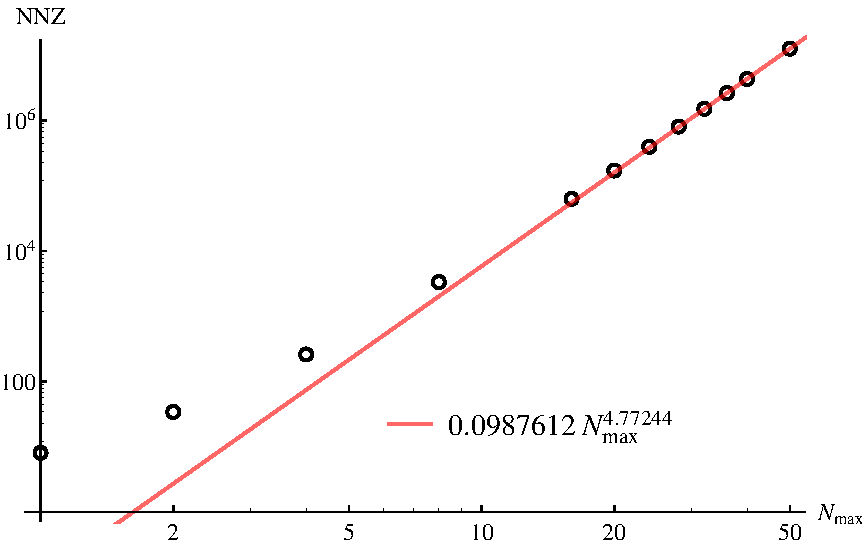
\includegraphics[width=.48\textwidth]{nnz.pdf}}
 \subfigure[The evaluation time as a function of $N_{\max}$]{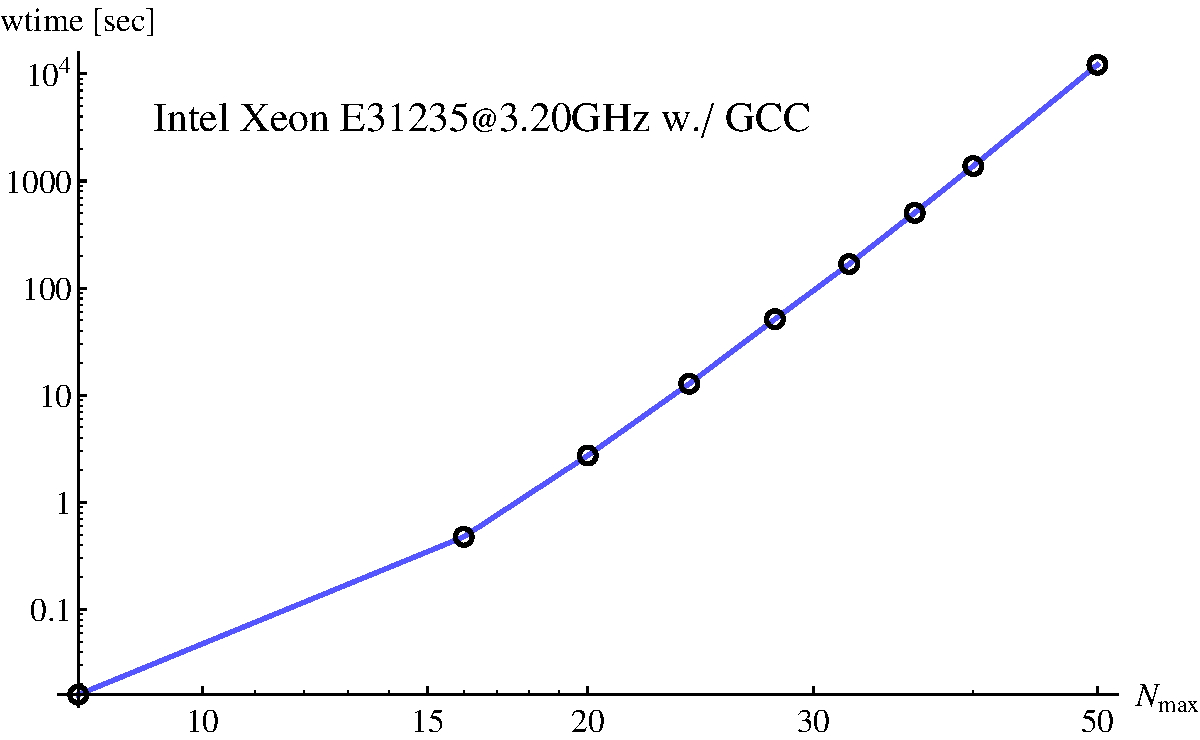
\includegraphics[width=.48\textwidth]{wtime.pdf}}
\caption{$r = 1$}
\end{figure}
%
\begin{figure}[ht]
 \centering 
 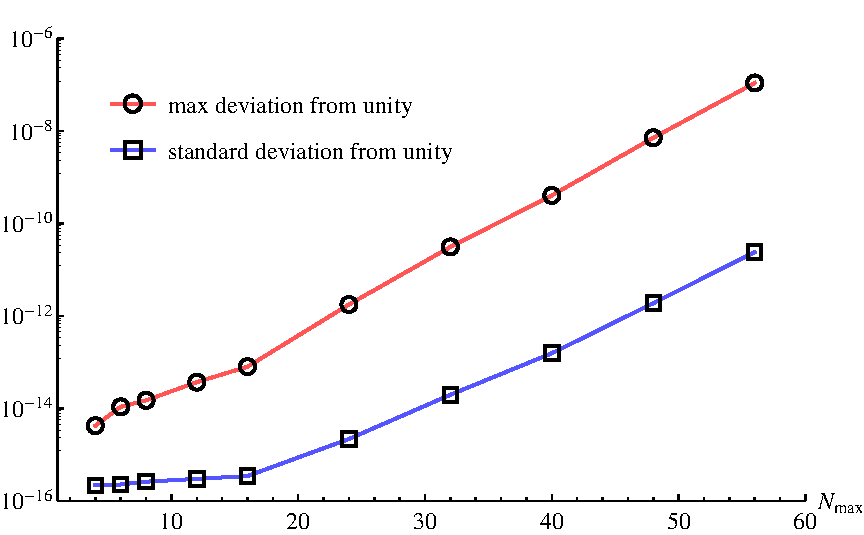
\includegraphics[width=.6\textwidth]{deviation.pdf}
 \caption{The standard and maximum derivation from unity for different $N_{\max}$ and $r=1$. 
The intermediate numbers are represented in \texttt{double precision}. }
\end{figure}

\paragraph{Higher Dimensions} The exponential generating function can be generalized to higher dimensional HO functions.


\begin{thebibliography}{9}

\bibitem{AnS.p376} M. Abramowitz and I. Stegun, eds. (1972),
Handbook of Mathematical Functions, with Formulas, Graphs and Tables, 
\textbf{9.6}, p.376,
New York: Dover Publication, ISBN 978-0-486-61272-0

\bibitem{AnS.p784} M. Abramowitz and I. Stegun, eds. (1972),
Handbook of Mathematical Functions, with Formulas, Graphs and Tables, 
\textbf{22.9}, p.784,
New York: Dover Publication, ISBN 978-0-486-61272-0



\end{thebibliography}

\end{document}
